\documentclass[fontsize=12pt,a4paper]{scrartcl}[2011/08/10]

\usepackage{listings}
\usepackage{courier}
\usepackage{graphicx}
\usepackage{float}
\usepackage{hyperref}

\title{Design of an UML tool with round-trip engineering for Java and implementation as a web application in Adobe Air}
\date{10.08.2011}
\author{Christoph Grundmann}

\begin{document}
\maketitle 
\newpage

\tableofcontents
\newpage 

\section{AlphaUML}
\subsection{Introduction}
AlphaUML is a simple UML tool for creating class diagrams, which supports round-trip engineering. It is designed for small projects and has its focus on being a learning tool for students. So it�s important that changes can be realized easily by a user, which will enhance the learning by doing process. Moreover AlphaUML is currently specialized for Java, so the parser supports only Java as programming language and dialogs are structured according to the Java syntax. Furthermore it has a fully integrated editor, which is useful to edit existing source code.

\subsection{Configuration}
\label{alphauml_options}
Some of the provided tools need to be configured. On the one hand the Java compiler \ref{javac} and on the other hand the JavaDoc generator \ref{javadoc} needs a specific file path, in which the executables are. In this case the "bin" directory of Java installation. Those paths can be set in the AlphaUML options. To open the options, navigate to the "File" menu and select the "Options" entry. Without the configuration, each of those programs throws an error and can't be executed.

\subsection{Projects}
\subsubsection{New Project}
\subsubsection{Load Existing Project}

\subsection{Console}
The console is a very useful tool to get information about the forward and reverse engineering process. It displays the current step of the executed process and catches errors. When a parsing error occurred the parser throws a message with all necessary information, like the Java file which causes the error and in which line and position it occurs. Furthermore it's able to execute the Java compiler \ref{javac} or the JavaDoc generator \ref{javadoc} by using their specific commands.

\begin{figure}[H]
\centering
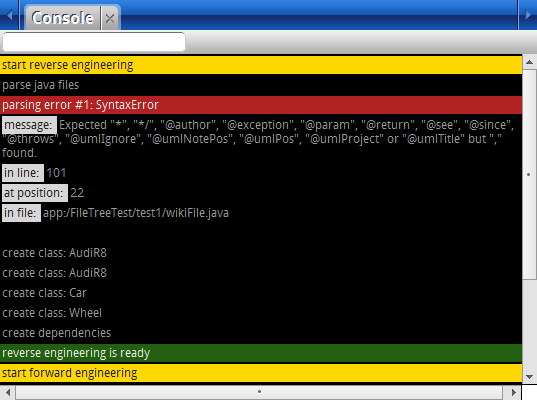
\includegraphics[scale=0.8]{images/console.png}
\caption{Console which showing the round-trip engineering process}
\end{figure}

\subsubsection{Java Compiler}
\label{javac}
To compile the current opened project, it's possible to execute the "javac" command via the command line of the console. Currently it saves the generated class file of an associated Java File in the "build" folder of the project, which will be found in the projects root. Moreover when the compiler throws an error, the console displays it. \newline To be able to execute the "javac" command the console needs the path of the Java compiler, which has to be set in the AlphaUML options \ref{alphauml_options}.

\paragraph{Command}
javac

\begin{figure}[H]
\centering
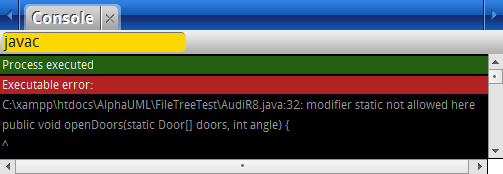
\includegraphics[scale=0.8]{images/console_javac.png}
\caption{Execution of the Java compiler}
\end{figure}
 
\subsubsection{JavaDoc Generator}
\label{javadoc}
It's also possible to generate documentation with the help of the JavaDoc generator. It collects each Java file of the project, which isn't ignored for those processes, and places the generated documentation into the "docs" folder of the projects root. \newline Like the "javac" command the "javadoc" command will be executed via the command line of the console and needs a correct configuration in the AlphaUML options \ref{alphauml_options}.

\paragraph{Command}
javadoc

\begin{figure}[H]
\centering
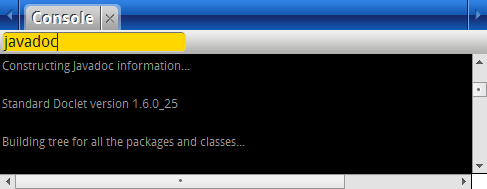
\includegraphics[scale=0.8]{images/console_javadoc.png}
\caption{Execution of the JavaDoc generator}
\end{figure}

\subsection{Code Editor}
The code editor, as a main feature of AlphaUML, is an advanced editor, with various functionalities, like the searching and replacing of code snippets and the syntax highlighting. The editor is based on Ace \ref{ace_editor} an open source editor written in JavaScript. Mainly Ace provides a huge collection of supported programming languages, like JavaScript, C/C++ or Java, but is optimized for editing JavaScript and CoffeeScript. So some features aren't supported in AlphaUML, like the showing of syntax errors. But this feature is available thru the round-trip engineering and compiling process, which errors are shown in the console.
The editor in AplhaUML is optimized for Java and text files and is able to save those files. If a new Java file will be created without a specific file path - for example after the code generation process � a file dialog will be opened, which can used to save those. Another feature, - which is useful if a user believes that the used font is too small, especially 'caused an amblyopic - can increment or decrement the font size. The last possibility is to search and replace parts of source code or other keywords, which will be necessary if a document includes a huge number of characters, and the user will search something special.

\begin{figure}[H]
\centering
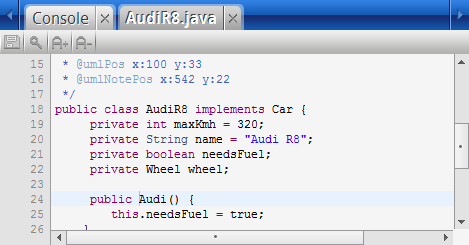
\includegraphics[scale=0.9]{images/editor.png}
\caption{View of the code editor}
\end{figure}

\subsection{Class Diagram Editor}
The class diagram editor is a small editor to draft class diagrams with a handful of tools to create classes, notes or for example generalizations. It simply consists of two components, the workspace and the toolbar, which gives access to each necessary tool. Moreover each tool is optimized for the Java programming language, to enhance Java developers.

\begin{figure}[H]
\centering
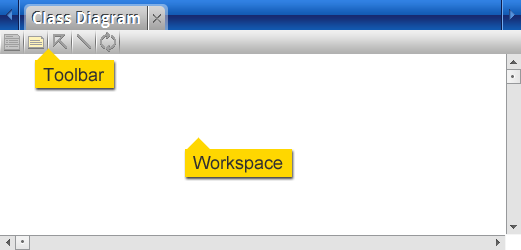
\includegraphics[scale=0.8]{images/class_diagram_editor.png}
\caption{Layout of the class diagram editor}
\end{figure}

\paragraph{Multiple usages of tools}
'Cause of the visual resemblance of some UML components, like the generalization- and a provided interface arrow, and the idea to provide a simple user interface without a huge collection of buttons, some tools will be used for multiple usages. Each tool uses depending on what type of action is registered, for example what type of classes are selected, their specific functionality. If a user use the "Add Generalization" tool and selects two classes a generalization will be created, but if the user selects an interface and a class, the tool adds a provided interface. To simplify the usage of those tools tooltips will be used to show each possible usage.

\paragraph{Supported UML notation elements}
The editor supports the following UML notation elements, which will be described in the next chapters.
 
\begin{enumerate}
\item Class \ref{class_desc}
\item Note \ref{note_desc}
\item Provided Interface \ref{provided_interface_desc}
\item Required Interface \ref{required_interface_desc}
\item Binary association \ref{association_desc}
\item Generalization \ref{generalization_desc}
\end{enumerate}

\subsubsection{Class}
\label{class_desc}
A class is a structural design for objects and contains attributes and operations, which describes its properties and functionalities. It is subdivided into 3 parts, a part for its name and stereotype or abstract declaration, another part for its attributes and at last a part for each operation of the class. To add a class the "Add Class" tool from the toolbar has to be selected, which allows placing a class into the workspace, by clicking on a specific place in it.

\begin{figure}[H]
\centering
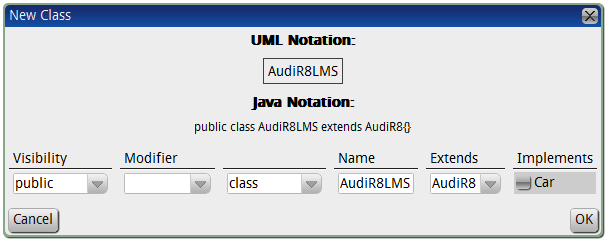
\includegraphics[scale=0.7]{images/add_class_dialog.png}
\caption{Dialog for adding a new class}
\end{figure}

After placing the class a dialog will be opened to configure the new class. It allows setting a class name, modifier or its visibility. Furthermore it's also possible to implement interfaces or to inherit from another class via the "Extends" option.\newline A special characteristic of each dialog, which will be used to add a class diagram-component, is its subdivision into 2 parts. On the top there is a preview, which shows the result of the current configuration as Java and a UML component. And at the bottom each component property can be set. So the user can see his changes directly.

\begin{figure}[H]
\centering
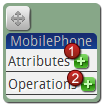
\includegraphics[scale=1]{images/class.png}
\caption{View of a class}
\label{desc_class}
\end{figure}

When a class is placed, it provides a various number of functionalities, like the adding of attributes or operations. The most mentionable functionality is the context menu of a class, which gives access to the �Edit Class� tool and gives possibilities to rename or remove the class. The context menu will be opened by a click on the class name. For adding a new attribute the plus icon beside the "Attribute" header - Figure \ref{desc_class} number 1 - has to be clicked, which opens the "Add Attribute" dialog.

\begin{figure}[H]
\centering
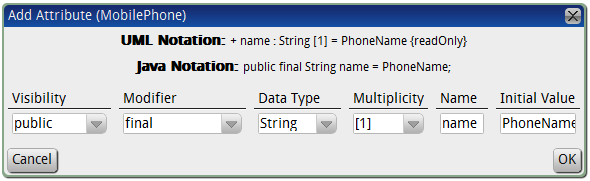
\includegraphics[scale=0.7]{images/add_attribute_dialog.png}
\caption{Dialog for adding a new attribute}
\end{figure}

Furthermore to create a new operation, the plus icon beside the "Operation" header  - Figure \ref{desc_class} number 2 -  is the way to go, to open the specific dialog.

\begin{figure}[H]
\centering
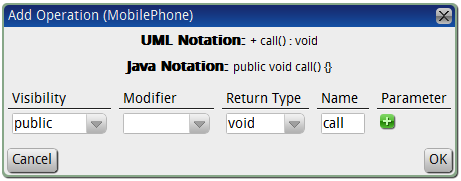
\includegraphics[scale=0.8]{images/add_operation_dialog.png}
\caption{Dialog for adding a new operation}
\end{figure}

Secondary to the typical operation properties, like the name, it's possible to add parameters via the "Add Operation" dialog. Parameters can also be added by using its plus icon, which is shown in any operation entry. In both cases the same dialog for adding parameters will be opened.

\begin{figure}[H]
\centering
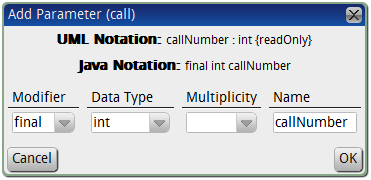
\includegraphics[scale=0.7]{images/add_parameter_dialog.png}
\caption{Dialog for adding a new parameter}
\end{figure}

Each operation and attribute is build-on so called tags, which are all clickable. A click on the name of an attribute or operation will open a context menu for configuring and deleting it. Each other tag is used for a quick access on its value. So it's possible to change the data type of an attribute by clicking on it and selecting another one from the opened context menu.

\begin{figure}[H]
\centering
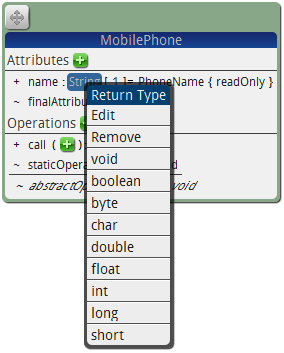
\includegraphics[scale=0.7]{images/attribute_datatype_quick_access.png}
\caption{Quick access}
\end{figure}

In some cases a Java modifier can't display as specific UML keyword. So it's commonly accepted to display attributes or operations with a different formation. Abstract class members will be shown with an italic font and static members are underlined. In addition final members use the \{readOnly\} property.

\begin{figure}[H]
\centering
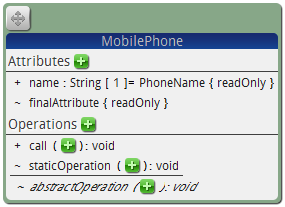
\includegraphics[scale=1]{images/class_modifier_views.png}
\caption{View of an final attribute and an abstract and static operation}
\end{figure}

\subsubsection{Note}
\label{note_desc}
A note is used to document a specific class. Its comment will be also used to generate with it a JavaDoc comment, during the forward engineering process \ref{forward_engineering_desc}. It's also possible to create a note without a relation to a class, which could be useful for small memos. To create a note the toolbar provides the "Add Note" tool, which allows placing a note into the workspace. If it's necessary to connect a note to a class the "Add Association" tool \ref{association_desc} will be used.

\subsubsection{Binary Association}
\label{association_desc}
When a class refers to another class, a binary association is used to visualize a relation between these classes. An association allows declaring the direction of the navigation, which defines in which class a reference, will be used. Moreover it's possible to set the role � name of its reference � and the multiplicity to set the min and max number of instances. The association name is only a notation element for an easier readability of the association and won't be used as a property of an instance.\newline To create a binary association the "Add Association" tool has to be activated. Then the two classes which will be in relation have to be selected. And after these steps a dialog will be opened, which provides the configuration of all necessary association properties.

\begin{figure}[H]
\centering
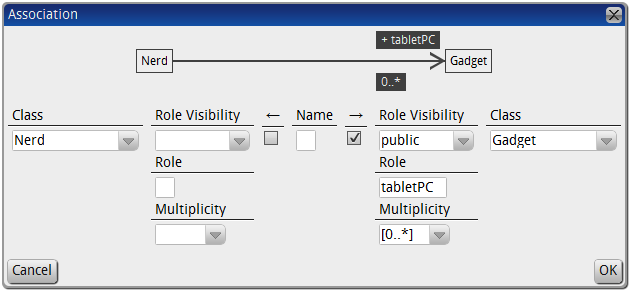
\includegraphics[scale=0.7]{images/add_association_dialog.png}
\caption{Dialog for adding a new binary association}
\end{figure}

\subsubsection{Generalization}
\label{generalization_desc}
A generalization describes a relation between a super- and a subclass and specifies that the subclass inherits from the superclass. So each attribute and operation of the superclass is also available in the subclass. It's also possible overwriting an operation, which can be handled by declaring the same operation with identical parameters like the one in the superclass. Otherwise the superclass operation will be used. To set a generalization the "Add Generalization" tool of the toolbar is used. After activating it the superclass has to be selected and then the subclass, which opens a dialog for setting it up. To edit this relation it's possible to click the generalization for opening a context menu, which allows the deletion of it also.

\begin{figure}[H]
\centering
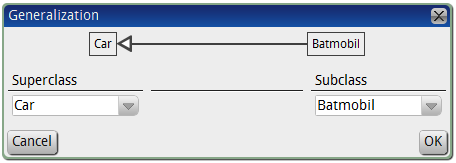
\includegraphics[scale=0.8]{images/add_generalization_dialog.png}
\caption{Dialog for adding a new generalization}
\end{figure}

\subsubsection{Required Interface}
\label{required_interface_desc}
An interface is a special kind of an abstract class, with the different that it's possible to inherit more than one interface. When a class uses a specific interface it's called a required interface, which can be set with the "Add Association" tool.

\begin{figure}[H]
\centering
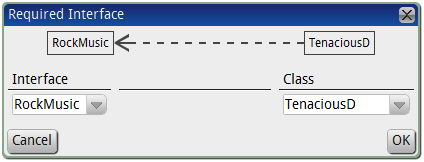
\includegraphics[scale=0.7]{images/add_required_interface_dialog.png}
\caption{Dialog for setting a new required interface}
\end{figure}

\subsubsection{Provided Interface}
\label{provided_interface_desc}
Moreover if a class inherits from an interface, it's called provided interface and can be set via the "Add Generalization" tool.

\begin{figure}[H]
\centering
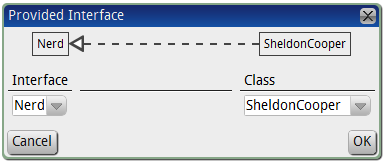
\includegraphics[scale=0.7]{images/add_provided_interface_dialog.png}
\caption{Dialog for setting a new provided interface}
\end{figure}

\subsubsection{Round-trip Engineering}
AlphaUML is able to generate a class diagram with help of the included Java source files of a project. Furthermore it's also possible to generate Java source code by analyzing a class diagram. These features are provided by the "Round-trip engineering" tool, and can be executed by a simple click on its specific button. If a diagram has to be built and another one is already exists in the parent tab, the old one will be removed, before a new one can be generated. So it's necessary to use a new tab, if the old diagram shouldn�t be removed. To read more over the round-trip engineering process show \ref{reverse_eng}.\newline
When Java sources files are generated from a diagram, they will be opened in blue accented code editor tabs, which signalize that their included documents aren�t saved yet and the documents are a result of the code generation. Furthermore the generated sources are including some special JavaDoc tags \ref{single_source}, which allow generating the identical diagram, after a restart of AlphaUML. The whole process with all necessary status information will be shown in the console tab, so the user gets an overview about the running process.

\newpage
\section{Implementation}
\subsection{Frameworks}
AlphaUML use a handful collection of libraries, which are used to improve the development process and allows the access to necessary system information, like the file system. Each framework is based on JavaScript, like AlphaUML, or supports JavaScript, so it�s theoretical possible to run the application in a web browser.

\subsubsection{Adobe Air}
With Adobe Air it�s possible to create web applications, which will be executed as a native application on a desktop PC or a tablet. It supports the development in JavaScript and HTML and provides a library, which gives access to some system side functions and programs, like the command console or the file system. Adobe Air use the WebKit engine to allow to execute a JavaScript application. This fact is also necessary to know for designing the application \ref{css}.

\subsubsection{Dojo Toolkit}
Dojo is an enhanced framework to build JavaScript web applications (apps) and provides a huge number of features, which speeds up the development. Furthermore it�s very useful to build JavaScript apps in an object oriented style. So it allows to use a package system, has a build-in class system, which simulates for example inheritance. In addition one of the most important features is the event system. So user-triggered events, like an "onclick" event can be caught. Moreover self-defined events can be thrown, which release specific functions to react on these events. 

\paragraph{Package System}
The package system is based on the folder structure of its project. So if a JavaScript file has the following path "lib/ui/Dialog.js" and it�s necessary to get access to the Dialog class, the dojo.require function has to include this file by setting its path as first parameter. The �require� function includes the file during the runtime, so it isn't necessary to load the whole script at the beginning, which will saving a lot of loading time.

\paragraph{Class System} 
The class system allows the declaration of classes and provides inheritance, which is necessary to develop software in object oriented style. So JavaScript is object oriented, but doesn't support to inherit from another object and it doesn't have classes. So Dojo uses some tricks to simulate these features.

\begin{itemize}
	\item{\href{http://javascript.crockford.com/prototypal.html}{Prototypal Inheritance}}
	\item{\href{http://javascript.crockford.com/inheritance.html}{Classical Inheritance}}
	\item{\href{http://javascript.crockford.com/private.html}{Private Members}}
\end{itemize}

\paragraph{Event System}
The use of events is particularly in JavaScript useful. So on the one hand it�s necessary to catch events from the DOM, which thrown by the user, for example on a click on a button. On the other hand self-defined events allow reacting in special cases, if an error is thrown or a specific routine is ready. In those cases a so called callback method can be executed, which can handle the result of the routine or shows for example an error message.

\subsubsection{PEG.js}
PEG.js is a JavaScript library, which generates a parser with the help of a specific grammar. So it�s possible to parse each programming language or to build a calculator, or something else. For more information show \ref{pegjs}.

\subsubsection{Ace}
\label{ace_editor}
Ace is a fast code editor with syntax highlighting and search- and replace-functions. It is fully developed in JavaScript and currently focused on JavaScript and CoffeeScript development, but allows using syntax highlighting for other languages, like Java, too.

\subsection{User Interface (UI)}
\subsubsection{Graphical Design}
\label{css}
To design the graphical user interface a style sheet language called cascading style sheets (CSS) is used. It describes the presentation semantics, which formats and sets the look of a HTML document. So it's possible to set the floating of elements, the size, the background color, specific fonts and many other formatting. In addition the style sheet is able to format each HTML element with an id or a class attribute. Classes will be accessed by a point and ids by a hash-symbol. If an element has a class called "Button" the selector looks like .Button and if an element has the id "dialog\_1" the selector will be \#dialog\_1. 'Cause of the HTML limitation, that an id is unique, the id selector will format only one element, wherever the class selector is able to format an unlimited number of elements.

\paragraph{JavaScript Specifics} 
In JavaScript CSS is also used for animations. So if the position of a DOM node will be changed, the element has to have an absolute position and the top and left property have to set. JavaScript writes that information in the DOM node and the web browser updates its view, which is need to realize a drag and drop feature or animations, like color and size changes.

\paragraph{Adobe Air Specifics} 
The Adobe Air HTML- and JavaScript engine is based on WebKit, an open source web browser engine. So it's necessary to know that some CSS features like text- or box-shadows need the prefix "-webkit-", which usage will shown in the example below.

\subsubsection{The basics of the GUI design}
\paragraph{UI Object}
Each UI element, like a tab or the file tree, inherits from a base class called ui.Object. This class provides the managing of event listener, the creation of a unique id or handles the deletion of the UI element. Furthermore it implies some useful utilities, like hiding or showing the UI element. But one of the most important features is the event manager. So it's necessary to unset each event listener, which listen to a removed DOM node. In addition the event manager provides the registration of new event listener for specific events and can deactivate, activate or remove each listener by name. Furthermore it's possible to activate or deactivate all listeners at the same time, what's necessary if a UI object will be destroyed. The "activate" and "deactivate" function can be overwritten to extend the functionality, by example to destroy the DOM node at deactivating. Another important feature is the generation of a unique id for the DOM node of the UI element. So the HTML standard defines that an id has to use once only. If two nodes have the same id, the JavaScript engine of the web-browser can't get access to both. To get a unique id the id-creator uses the class name as base and searches for other nodes of that class, counts each appearance and appends the counter to the class name. The last mentionable function of the base class is the deletion handling. To be sure that each registered event listener and each used UI element of an UI element, like a button of a dialog, including the DOM node will be destroyed, the base class has a specific destroy function, which handles the "garbage collection". To initialize an UI object a function called "create" will be used. It generates a unique id, places the DOM node and sets up all necessary event listeners. A UI object has a specific uitype, which will be used to identify a DOM node as a UI element. It will be set as a HTML attribute and can be accessed on a catch event.

\paragraph{Window}
On the top of the GUI the window object manages the resizing and the full-screen mode of the Adobe Air window. It contains a collection of frames, which will be placed and resized with the help of the current window properties.

\paragraph{Frame}
A frame is the main actor in handling tabs and its content. In addition it resizes the tab content, like the Java editor or the file tree, and allows opening new tabs. In addition it handles the replacing and deletion of tabs. To drag a tab into another frame, the tab, its content and context menu will be removed from the old frame and replaced into the new one. In this case only the DOM nodes will be destroyed, but the Meta data - like the source code of a specific editor tab - because it�s necessary to be able to recreate the tab.

\paragraph{Tab}
A tab is only a draggable button, which references to its content and context menu. It's used to show or hide a specific content, like a code editor. A tab is subdivided into 3 parts. At first the tab themselves, which handles the create- and destroy-process of its content and context menu. In addition it starts its replacing process, which will be handled by the parent frame, if a user begins to drag the tab.

\paragraph{Context Menu}
The next part of a tab is its context menu. The context menu holds a collection of buttons, which can be used to execute specific functions of a tab. For example the editor tab has buttons to save its current document or to resize the font size.

\paragraph{Content}
The last part is the content object. It provides the access of some tools, like the class diagram editor, a Java editor or a file tree.

\begin{figure}[H]
\centering
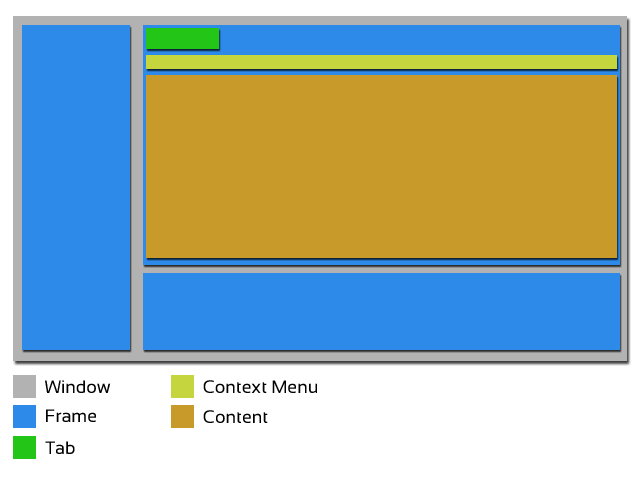
\includegraphics[scale=0.5]{images/gui_design.png}
\end{figure}

\subsubsection{Additional GUI components}
The GUI framework provides a number of UI components, which will be necessary for an application. The following list shows each available component.

\begin{description}
	\item[Dialog]
	\item[Tooltip]
	\item[MouseInfo]
\end{description}

\subsection{Single Page Web App}
Usually a web application is using a handful of HTML pages for rendering its content. A single page web app has only one HTML document, which will be updated by some JavaScript functions. So it's possible to place, replace or remove DOM nodes during the runtime. Another characteristic of a web application is its fragmentation into backend - usually server-side - and frontend - client-side -, which concept is also be used in a single page web app. But AlphaUML is designed as a single page web app without a backend, which could be used for parsing or for getting access to files from storage. All these functionality is transferred to the frontend, so each process will be executed on the client side. To realize that concept, the compiler and any other feature is completely written in JavaScript. In addition Adobe Air is used to get access to functionalities, which JavaScript isn't allowed to. For example JavaScript can't get access to the file system of a client, 'cause of security reasons. In this case Adobe Air is the way to go.

\subsection{Single Source Publishing}
\label{single_source}
To avoid project files AlphaUML follows the single source publishing concept. It allows using the context of a document in different ways. In this case a Java document is used to initialize a project or to generate a class-diagram, without losing its specific usage as source file. So each necessary project-information will be saved into existing Java files. This is realized by using a various selection of specific JavaDoc tags, which begin with the @uml prefix. To use those tags the compiler is optimized to read them during the reverse engineering process \ref{reverse_eng}. Furthermore the UML specific tags will be generated by the code generator \ref{forward_eng}. 

\begin{figure}[H]
\centering
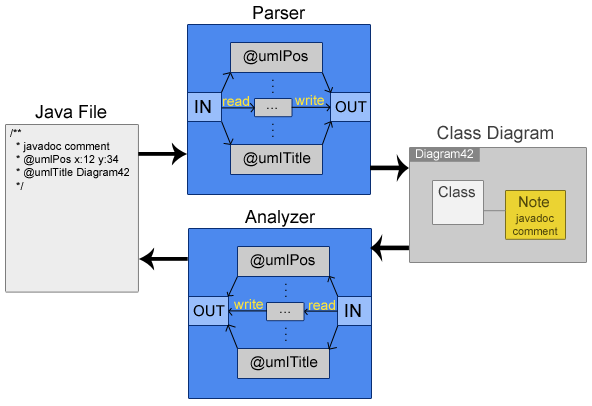
\includegraphics[scale=0.7]{images/single_source.png}
\end{figure}

\subsubsection{Class Diagram Specifics}
\paragraph{@umlPos x:42 y:42}
The position-tag defines the position - in pixel - of a class in the class diagram.

\paragraph{@umlNotePos x:42 y:42}
If a class has a comment included, the position of the note will be stored in the note-position-tag. In addition if more than one note is connected to a class, the position of the first note will be used.

\paragraph{@umlTitle title-text}
The title-tag defines the title of the last generated class-digram.

\paragraph{JavaDoc Comment}
A special case is the JavaDoc comment itself. It is used to generate notes, which will be pinned to its associated class. In addition if the user creates a new note, the code generator uses as JavaDoc class comment. Moreover multiple usages of notes are allowed, so each note comment will be merged to one comment.

\subsubsection{Project Specifics}
\paragraph{@umlProject root:path/folder main:path/file.java}
The project-tag is used to define the project main file. It includes the relative root path and the main Java file with an absolute path.

\paragraph{@umlIgnore path}
To exclude specific files or folder, the ignore-tag allows ignoring those for the class diagram generation. That could be necessary if only a part of files should include in the class diagram, or if some Java files don�t follow the java syntax completely, 'cause of its use to store only Java snippets.

\newpage
\section{Round-trip engineering}
Today's complexity of software requires the use of diagrams that will describe the structure of programs and how the internal processes communicate, during and primary at the beginning of the development. Moreover for object oriented languages like Java, the UML standard is the way to go, because of its focus for the object oriented developing of software.  
Structure diagrams, like the class diagram, have the capability to generate source code by analyzing it. In addition it's possible to create a class diagram with the help of source code. 
The creation of Java source code from a class diagram is called forward engineering, whereas the creation of a class diagram from the Java source code is called reverse engineering. The whole technique is known as round trip engineering. So round trip engineering allows keeping the consistency between diagrams and source code.

\subsection{Reverse engineering}
\label{reverse_eng}
To generate a class diagram with the help of Java source code, a parser is needed to interpret the grammatical structure of it. Usually a program doesn�t understand the grammatical structure of an input like a string before it is interpreted. The first step in interpreting the source code a parser converts it into a specific data format, in this case into a JSON object, which can use to interpret the grammatical structure. After that step the new output can be used to generate the class diagram. Classes can easily instantiate by reading the JavaScript friendly output, where the relations need to be interpreted.

\subsubsection{Parser}
\label{pegjs} 
AlphaUML uses �PEG.js�, a Java parser that is completely written in JavaScript, to parse Java source code into a JSON object. It allows converting a string, by using a specific language grammar, into any output format. The grammar describes the Java language and defines the output. It follows specific rules similar to regular expressions to match the input with the Java grammar. 
Furthermore it allows manipulating the output of each expression by using JavaScript as a so called �action�. In this case an action is used to convert the expression result to a JSON object. But in some cases an empty string returns if an expression is optional and it doesn�t match. Then the empty string will be replaced with null to catch missing matches in the processing to a class diagram.

\subsubsection{Parser grammar rules}
PEG.js provides some rules which are necessary to write an own grammar. A collection of the most common rules will be described below. In addition a small grammar example with explanation after the rules shows how they are used.

\paragraph*{\textbf{"literal" or 'literal'}}$\;$ \\
Return the literal string on matching.

\paragraph*{\textbf{.}}$\;$ \\
Return one character as a string.

\paragraph*{\textbf{\lbrack characters\rbrack}}$\;$ \\
Return one character of the bracket contained set.

\paragraph*{\textbf{rule}}$\;$ \\
It describes a fully expression that can use in other rules or expressions

\paragraph*{\textbf{(expression)}}$\;$ \\
It allows the declaration of a subexpression to encapsulate it. It�s similar to a rule and is necessary to set an expression optional.

\paragraph*{\textbf{expression *}}$\;$ \\
Zero or more match results allowed. Returns the result as an array.

\paragraph*{\textbf{expression +}}$\;$ \\
One or more match results necessary. If the input doesn't match it returns a parsing error.

\paragraph*{\textbf{expression ?}}$\;$ \\
It allows optional expressions. On succeeding the match result returns, otherwise it returns an empty string.

\paragraph*{\textbf{! expression}}$\;$ \\
It forbids a specific expression.

\paragraph*{\textbf{label : expression}}$\;$ \\
A label stores the match result into a specific variable that has the same name. It can be used in an action to get access of the stored result.

\paragraph*{\textbf{expression \{ action \}}}$\;$ \\
An action is a JavaScript snippet that will be executed 'cause the match is successful. It has the access to each labeled expression of its expression and allows the manipulation of the match result.

\paragraph*{\textbf{expression\_1 expression\_2 \dots expression\_n}}$\;$ \\
A sequence of expression is allowed and returns their results as an array.

\paragraph*{\textbf{expression\_1 / expression\_2 / \dots / expression\_n}}$\;$ \\
It allows to create an OR function. It tries to match with one of the given expressions.

\subsubsection{Parser grammar example}
The following example shows a rule called DataType which is used for parsing a data type. It matches primitive data types, generic types or array types. Each information will return as a JSON object, formatted by the action. The DataTypeKeyword rule provides a collection of data types and allows each possible java identifier (Identifier) as data type, so user-defined objects are possible. The Generic and Array rules are optional and return an empty string on miss.

\lstset{
	language=HTML, 
	numbers=left,
	numberstyle=\tiny,
	stepnumber=1
}

\begin{lstlisting}[caption={list of data type keywords}, frame=single]
DataTypeKeyword = (
        "boolean"
	/   "byte"
	/   "char"
	/   "double"
	/   "enum"
	/   "float"
	/   "int"
	/   "long"
	/   "short"
	/   "void"
	/   Identifier
)
\end{lstlisting}

\begin{lstlisting}[caption={data type rule}, frame=single]
DataType =
    $d:DataTypeKeyword __
    $g:($g:Generic __ {return $g;})?
    $a:($a:Array __ {return $a;})?
    {
        return {
            generic: $g !== "" ? $g : null,
            array: $a !== "" ? $a : false,
            dataType: $d
        };
    }
\end{lstlisting}

\subsubsection{Parser output}
\label{json} 
The produced output from the source code will be used to generate the class diagram. The JSON format of the output makes the next process easier, so it represents a specific logical structure and allows the immediate access to all necessary information about the parsed Java program.
The output provides, for example, the info about used libraries, the class package, all class methods or variables to generate the class diagram. In addition the JavaDoc is available and will be pinned as note at the specific class in the diagram.
The following JSON sample gives an overview about the output format and shows each possible fields like the "package" or "classes" fields.

\begin{lstlisting}[caption={file output}, frame=single]
{
   "package": "packageName",
   "imports": ["path"],
   "classes": []
}
\end{lstlisting}

\begin{lstlisting}[caption={classes output}, frame=single]
"classes": [
     {
        "type": "interface",
        "javaDoc": null,
        "visibility": "public",
        "name": "className",
        "extend": "superClass",
        "implement": [
            "interfaceName"
        ],
        "body": {
            "variable": [],
            "method": []
        }
    }
]
\end{lstlisting}

\begin{lstlisting}[caption={variable output}, frame=single]
"variable": [
    {
        "type": "variable",
        "javaDoc": null,
        "name": "varName",
        "visibility": "public",
        "modifier": [
            "static",
            "final"
        ],
        "array": false,
        "generic": null,
        "dataType": "int",
        "value": "42"
    }
]
\end{lstlisting}

\begin{lstlisting}[caption={method output}, frame=single]
"method": [
    {
        "type": "method",
        "javaDoc": {},
        "name": "methodName",
        "visibility": "public",
        "modifier": [],
        "generic": null,
        "array": true,
        "dataType": "String",
        "parameter": [
            {
                "type": "parameter",
                "modifier": ["static"],
                "generic": "T",
                "array": false,
                "dataType": "Object",
                "name": "paramterName"
            }
        ],
        "body": "methodBody"
    }
]
\end{lstlisting}

\begin{lstlisting}[caption={JavaDoc output}, frame=single]
"javaDoc": {
     "since": [
        {
           "tag": "since",
           "description": "desc"
        }
     ],
     "throws": [
        {
           "tag": "throws",
           "classname": "className",
           "description": "desc"
        }
     ],
     "exception": [
        {
           "tag": "exception",
           "classname": "className",
           "description": "desc"
        }
     ],
     "param": [
        {
           "tag": "param",
           "name": "paramName",
           "description": "desc"
        }
     ],
     "return": [
        {
           "tag": "return",
           "description": "desc"
        }
     ],
     "see": [
        {
           "tag": "see",
           "description": "desc"
        }
     ]
}
\end{lstlisting}

\subsubsection{Class diagram generation}
After parsing the Java source code the new data structure can be used to build a class diagram, which visualize the logical structure of its program. The process which builds the class diagram is subdivided into 3 parts. In the first step each class with all selected info - like the name, its variables and operations - will be created. If two classes with the same name exist, the name of the second class will be renamed. In this case each relation which has a reference on its class name could not be created anymore. During the first step any information which is needed for generalizations or the relations of provided interfaces will be stored. So it is not necessary to read the parser output twice. With the help of the stored information each generalization and all relations of provided interfaces can be created in step two. The last step needs the interpretation of each created class. To generate associations or the relations of required interfaces, each attribute of each class has to be analyzed. If an attribute has a data type of an existing class, it's a candidate for an association. In this case this class will be analyzed, too, to figure out whether the association has bidirectional navigation.

\subsection{Forward engineering}
\label{forward_eng}
To generate the source code from an existing class diagram, it's essential to analyze each available class and connector, like generalizations or associations. The analyzing process will be handled from the classes themselves. So a class contains all necessary information and can handle it without an additional effort. Operations, parameter, attributes and classes own a method called \textit{getJSON()} that creates an output which is identical to the parser output \ref{json} and will be used to generate the source code. Furthermore it gets the relations between classes, so an additional process isn't necessary. On getting each declared attribute, associations of the two classes and each required interface will be collected and set as attribute. Moreover if an interface extends another interface it will set as superclass and declare with the extend keyword, in the other case if a class provides an interface the implements keyword will be used. The following sections explain each available relation and their implementation. 

\subsubsection{Generalization}
\label{generalization}
If a class inherits from another class the subclass has to signalize the relation with the keyword "extends" in its declaration. In addition each operation and attribute which exists in the superclass doesn't need to be implemented into the subclass twice. If the user defines an operation which has the same name and parameter list of another one in the superclass, the superclass operation will be overwritten. To execute the method of the superclass Java contains the "super" keyword which is a reference on its superclass.

\begin{figure}[H]
\centering
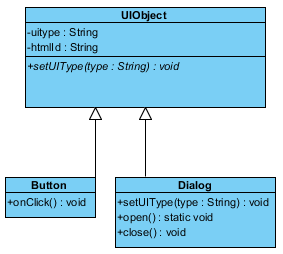
\includegraphics[scale=0.8]{images/example_generalization.png}
\end{figure}

The class diagram shows the superclass "UIObject" and two subclasses which inherit from it. Moreover the class "Dialog" overrides the operation "setUIType" and implements some other methods.

\lstset{
	language=Java, 
	numbers=left,
	numberstyle=\tiny,
	stepnumber=1
}

\begin{lstlisting}[caption={The following code snippet shows the result of the code generation.}, frame=single]
public class UIObject {
	private String uitype;
	private String htmlId;
	
	public void setUIType(String type) {}
}

public class Button extends UIObject {
	public void onClick() {}
}

public class Dialog extends UIObject {
	public void setUIType(String type) {}

	public void open() {}

	public void close() {}
}
\end{lstlisting}

\subsubsection{Binary association}
A binary association specifies a semantic relationship between two classes. So each class knew about the other one and is able to interact or communicate with it. An association provides a collection of properties, which are important to interpret for the code generation. First of all the multiplicity of a class defines the frequency of occurrence. If a multiplicity is declared as \lbrack 1..5\rbrack  the class has to declare once and can be declared at most five time. In the source code a multiplicity represents an array if a class can declare more than one time. Otherwise it�s a simple variable. Furthermore the role of a class gives the instance of itself a specific name. So if a role is set, the variable gets the name of it. In addition it's possible to set the visibility of a role. The last necessary association property is the navigation. An arrow visualizes the direction of the navigation and specify in which class the other one will be accessible. The bidirectional navigation allows the navigation in both directions.

\begin{figure}[H]
\centering
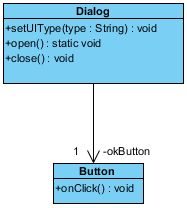
\includegraphics[scale=0.8]{images/example_association.png}
\end{figure}

In this example the dialog implements a button which is called "okButton". In addition it's accessible in the dialog class only, 'cause of the "private" visibility. Moreover the multiplicity of 1 provides that only one button can instantiate.

\begin{lstlisting}[caption={The following code snippet shows the result of the code generation.}, frame=single]
public class Button {
	public void onClick() {}
}

public class Dialog {
	private Button okButton;
	
	public void setUIType(String type) {}

	public void open() {}

	public void close() {}
}
\end{lstlisting}

\subsubsection{Provided interfaces}
Provided interfaces are like generalizations with abstract classes. Each operation will be inherited and has to overwrite in the subclass. The only two differences are the "implements" keyword � instead of the �extends� keyword � which is use for inheritance and the fact that it's possible to implement more than one interface. When using more than one interface, each interface will be separated by a comma, at its declaration. An interface provides abstract methods only, which order a specific realization of the class that inherits from it.

\begin{figure}[H]
\centering
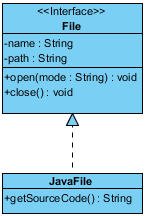
\includegraphics[scale=0.8]{images/example_provided_interface.png}
\end{figure}

This UML diagram shows the class "JavaFile", which use the "File" interface for a standardized communication. To use the interface the interface visibility is set to "public" and the class, which implements it, will redefine each operation of the interface.  

\begin{lstlisting}[caption={The following code snippet shows the result of the code generation.}, frame=single]
public interface File {
	private String name;
	private String path;
	
	public void open(String mode);

	public void close();
}

public class JavaFile implements File {
	public String getSourceCode() {}
	
	public void open(String mode);

	public void close();
}
\end{lstlisting}

\subsubsection{Required interfaces}
A required interface allows the communication between a class and another class which implements an interface. If more than one class inherit from a specific interface it's possible to get access to each of them in the same way. This means that all classes which communicate through that interface are constrained of its operations. So it would throw exceptions if one of those operations is changed. A required interface will be declared as an attribute and can be initialized by any constructor of classes which implement the interface.

\begin{figure}[H]
\centering
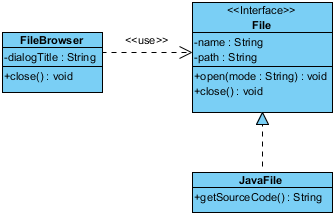
\includegraphics[scale=0.8]{images/example_required_interface.png}
\end{figure}

In this example the FileBrowser use an interface to get a standardized access to each file type, which implements the "File" interface. In this case a file could be a JavaFile or maybe a TextFile, or something else. The required interface will be declared as an attribute with the data type "File" and can be initialized with the JavaFile constructor \textit{private File javaFile = new JavaFile("read");}. But the code generator sets only the attribute. 

\begin{lstlisting}[caption={The following code snippet shows the result of the code generation.}, frame=single]
public interface File {
	private String name;
	private String path;
	
	public void open(String mode);

	public void close();
}

public class FileBrowser {	
	private String dialogTitle;
	private File _file;

	public void close() {}
}
\end{lstlisting}

\subsubsection{Extended interfaces}
If an interface will be extended, a generalization \ref{generalization} has to be used. That includes the UML generalization arrow and on the Java side, the use of the �extends� keyword.

\begin{figure}[H]
\centering
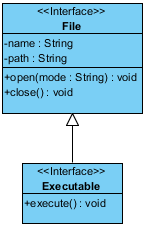
\includegraphics[scale=0.8]{images/example_extended_interface.png}
\end{figure}

In this case the Executable interface extends the File interface with the execute function.

\begin{lstlisting}[caption={The following code snippet shows the result of the code generation.}, frame=single]
public interface File {
	private String name;
	private String path;
	
	public void open(String mode);

	public void close();
}

public interface Executable extends File {
	public void execute() {}
}
\end{lstlisting}

\end{document}